\documentclass[12pt]{article}

\usepackage[utf8]{inputenc}
\usepackage{amsmath}
\usepackage{amssymb}
\usepackage{caption}
\usepackage{color}
\usepackage{float}
\usepackage{graphicx}
\usepackage{listings}
\usepackage{physics}
\usepackage{tikz}
\usepackage{listings}
\usepackage{subfiles}
\usepackage{enumerate}

\setlength{\parindent}{5em}
\setlength{\parskip}{1em}
\renewcommand{\baselinestretch}{1.5}

\title{	
	\textbf{CSE-315 Microprocessor}
	\endgraf\bigskip
}

\author{
	\Large{Waqar Hassan Khan}\\
	\Large{Student ID : 1505107}
}

\date{}

\begin{document}

\maketitle

%---------------------------------------------------------------------------------------
%lecture-1
\section{Chapter-9 : 8086/8088 specification}

\begin{itemize}
	\item virtually no differences between these two microprocessors. Both are packaged in 40-pin dual in-line package.
	
	\item\textbf{8086:}16 bit microprocessor with a 16bit data bus(A0-A15)\\
	\textbf{8088:}16 bit microprocessor with a 8bit data bus(A0-A7)\\
	major difference between 8086 and 8088.
	
	\item Minor differences\\
	\textbf{8086:}M/$\overline{IO}$;\textbf{8088:}IO/$\overline{M}$\\
	PIN34:-\textbf{8086:}$\overline{BHE}$/S7;\textbf{8088:}SS0\\
	
	\item power supply requirements:\\
	+5v with a supply voltage tolerance of $+-10\%$\\
	both 32F to 180F\\
	8086 and 8088 have 340 and 360 mA.
	
	\textbf{figures in the book}
	
	\subsection{Pin Connection}
	\begin{itemize}
		\item \textbf{AD7-AD0:}\\
		-8088 address/data bus lines\\
		-multiplexed address data bus\\
		-rightmost 8 bits of the memory address or I/O port whenever ALE=1 or ALE=0\\
		-high impedance state during hold acknowledge.\\
		
		\item \textbf{A15-A8:} \\
		-8088 address bus\\
		-high impedance state during hold acknowledge.\\
		
		\item \textbf{AD15-AD8:}\\
		-8086 address/data bus lines.\\
		-contains address bits when ALE=1\\
		-high impedance state during hold acknowledge.\\
		
		\item \textbf{A19/S6-A16/S3:}\\
		-multiplexed address/data bus lines\\
		-high impedance state during hold acknowledge.\\
		
		\item\textbf{S6:} always 0\\
		\item\textbf{S5:} indicated the condition of \textbf{\textcolor{red}{IF}} flag\\
		
		\begin{table}[H]
			\centering
			\begin{tabular}{|c|c|c|}
				\hline
				S4 & S3 & indicate segment accessed  during current bus cycle\\\hline
				
				0 & 0 & extra segment\\\hline
				0 & 1 & stack segment\\\hline
				1 & 0 & code or no segment\\\hline
				1 & 1 & data segment\\\hline
			\end{tabular}
		\end{table}
	
		\item -$\overline{RD}:$ if it is 0 then the data bus becomes receptive to data from memory or i/o devices connected to the system.\\
		-high impedance state during hold acknowledge.\\
		
		\item\textbf{READY:}\\
		-enters into wait state and remains idle if 0\\
		-no effect on operations of microprocessor if this pin is in logic state 1.\\
		
		\item\textbf{INTR:}\\
		-used to request a h/w interrupt.\\
		-if INTR=1 when IF=1 then microprocessor enters an interrupt acknowledge cycle after completion of current instruction\\
		
		\item\textbf{NMI:}\\
		-non maskable interrupt pin.\\
		-similar to INTR except do not check IF flag.\\
		
		\item$\overline{\textbf{TEST}}:$\\
		-an input that is tested by \textbf{wait} instruction.
		-if it is 0, the \textbf{WAIT} functions as \textbf{NOP}.\\
		-if 1 then \textbf{WAIT} waits for   $\overline{\textbf{TEST}}$ to become logic 0.\\
	\end{itemize}
\end{itemize}
%---------------------------------------------------------------------------------------

\newpage

%---------------------------------------------------------------------------------------
%lecture-2
\section{Chapter-9 : 8086/8088 specification}
\begin{itemize}
	\item\textbf{NMI:}\\
	-non-maskable interrupt pin \\
	-similar to INTR except that NMI does not check IF flag.\\
	
	\item\textbf{RESET:}\\
	-causes the microprocessor to reset if this pin remains high for a minimum of 4 clocking periods.\\
	-whenever the microprocessor  gets reset, it begins executing instructions at memory location FFFF0H and disables future interrupts by clearing IF.\\
	
	\item\textbf{CLK:}\\
	-provides the base timing signal to the microprocessor.\\
	-clock signal must have at least 33\% duty cycle(high for $\frac{1}{3}$ rd and low for $\frac{2}{3}$ of the period)\\
	
	\item\text{VCC}\\
	-power supply input\\
	-provides +5V \\
	
	\item\textbf{GND:}- 2 pins, both must be connected to ground.\\
	
	\item\textbf{MN/$\overline{MX}$}:-selects either minimum mode or maximum mode operations of microprocessor.\\
	
	\item\textbf{$\overline{BHE}$/S7}-both high enable.
	-use in 8086 to enable the most significant data bus bits(D15-D8) during a read or write\\
	-the state of S7 is always a logic1
	
	\subsection{Minimum Mode Pins}
	\begin{itemize}
		\item\textbf{IO/$\overline{M}$ or M/$\overline{IO}$}\\
		-selects memory or i/o 
		-indicates that microprocessors address\\ bus contains either a memory address or an i/o port address.\\
		-high impedance state during a hold acknowledge.\\ 
		
		\item \textbf{$\overline{WR}$:} \\
		-indicates that microprocessor is outputting data to a memory or io device.\\
		-data bus contains valid data for memory or io during the time, WR remains 0.\\
		
		\item \textbf{$\overline{INTA}$:} \\
		-a response to the INTR input pin.\\
		-used to gate the interrupt vector number onto the data bus in response to an interrupt request.\\
		
		\item \textbf{$\overline{ALE}$:} \\
		-address latch enable.\\
		-indicates that the microprocessor address/data bus contains address information.\\
		-the address can be a memory address or an i/o port.\\
		-does not float during a hold acknowledge.\\
		
		\item\textbf{DT/$\overline{R}$:} - data transmit or receive.\\
		-indicates that microprocessors data bus is transmitting(DT/$overline{R}$=1) or receiving(DT/$overline{R}$=(DT/$overline{R}$=0) data.\\
		-used to enable external data bus buffers.\\
		
		\item\textbf{DEN:}-data bus enable\\
		-activates external data bus buffers.\\
		
		\item\textbf{HOLD:} - requests a direct memory access (DMA).\\
		-if it is logic 1, microprocessor stops executing s/w and places its address, data and control bus at high impedance state.\\
		-if it is a logic 0, the microprocessor executes s/w normally.\\
		
		\item\textbf{HLDA:} - hold acknowledge\\
		-indicates that the microprocessor has entered the hold state.\\
		
		\item\textbf{$\overline{SS0}$} - equivalent to the S0 pin in the maximum mode operation.\\
		-it is combined with IO/$\overline{M}$ and DT/$\overline{R}$ to decode function of the current bus cycle.
		  
	\end{itemize}  

	\begin{table}[H]
		\centering
		\begin{tabular}{|c|c|c|c|}
			\hline
			IO/$\overline{M}$ & DT/$\overline{R}$ & $\overline{SS0}$ & \textbf{function}\\\hline
			
			0 & 0 & 0 & interrupt acknowledge\\\hline
			0 & 0 & 1 & memory card\\\hline
			0 & 1 & 1 & memory write\\\hline
			0 & 1 & 1 & halt\\\hline
			1 & 0 & 0 & opcode fetch\\\hline
			1 & 0 & 1 & I/O read\\\hline
			1 & 1 & 0 & I/O write\\\hline
			1 & 1 & 1 & passive/inactive\\\hline
		\end{tabular}
		\caption{bus cycle status(8088)[minimum mode]}
	\end{table}

		\begin{table}[H]
		\centering
		\begin{tabular}{|c|c|c|c|}
			\hline
			I$\overline{S2}$ & $\overline{S1}$ & $\overline{S0}$ & \textbf{function}\\\hline
			
			0 & 0 & 0 & interrupt acknowledge\\\hline
			0 & 0 & 1 & I/O card\\\hline
			0 & 1 & 1 & I/O write\\\hline
			0 & 1 & 1 & halt\\\hline
			1 & 0 & 0 & opcode fetch\\\hline
			1 & 0 & 1 & memory read\\\hline
			1 & 1 & 0 & memory write\\\hline
			1 & 1 & 1 & passive\\\hline
		\end{tabular}
		\caption{bus control functions generated by the bus controller 8088[maximum mode]}
	\end{table}
\end{itemize}
%---------------------------------------------------------------------------------------

\newpage

%---------------------------------------------------------------------------------------
%lecture-3
\section{8086/8088 hardware specifications}
\textbf{Maximum Mode Pins:} for using with external co-processors \\
\begin{itemize}
	\item$\overline{S2}, \overline{S1}, \overline{S0}$ - indicate the function of current bus cycle.\\
	-normally decoded 8288 bus controller.\\
	
	\item $\overline{R1}/\overline{GT1} and \overline{R0}/\overline{GT0}$ - request/grant pins \\
	-requests direct memory access(DMA)\\
	-used to both request and grant DMA operation.\\
	
	\item\textbf{$\overline{LOCK}$} - used to lock peripheral off the system.\\
	
	\item \textbf{OS1 and OS2} - queue status bit.\\
	-show status of the internal instruction queue.\\
	-accessed by numeric co-processor(8087)\\
	
	\begin{table}[H]
		\centering
		\begin{tabular}{|c|c|c|}
			\hline
			QS1 & QSA & Function\\\hline
			0 & 0 & queue is idle\\\hline
			0 & 1 & first byte of opcode\\\hline
			1 & 0 & queue is empty\\\hline
			1 & 1 & subsequent byte of opcode\\\hline
		\end{tabular}
	\end{table} 
\end{itemize}

\subsection{clock generator-8284A}
\begin{figure}[H]
	\centering
	\captionsetup{justification=centering}
	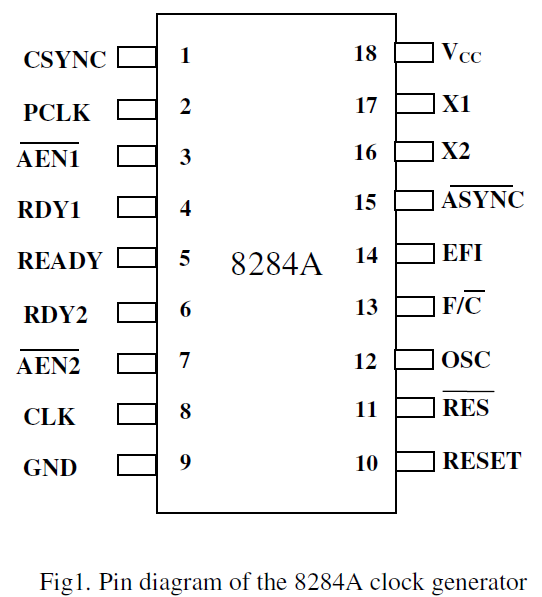
\includegraphics[width = 0.5\textwidth]{image/8284A.png}
	\caption{
		8284A clock generator
	}
	\label{fig:fib}
	
\end{figure}

\begin{itemize}
	\item \textbf{Basic functions:}\\
	-clock generation\\
	-RESET synchronization\\
	-READY synchronization\\
	-TTL-level peripheral clk signals\\
	
	\item\textbf{pin functions}\\
	
	\item\textbf{AEN1 and AEN2 (address enable)} - qualify the bus ready signals RDY1 and RDY2 respectively.\\
	-wait states are generated by the READY pin of microprocessor, which is controlled by $\overline{AEN1}$ and $\overline{AEN2}$
	
	\item\textbf{RDY1 and RDY2} - Bus ready inputs.\\
	-cause wait states in conjunction with $\overline{AEN1}$ and $\overline{AEN2}$ pins.\\
	
	\item$\overline{\textbf{ASYNC}}:$ - READY synchronization.\\
	-selects either one or two stages of synchronization for RDY1 and RDY2 inputs.\\
	
	\item\textbf{READY} - an output pin that connects to microprocessors READY input.\\
	-synchronized with RDY1 and RDY2 inputs.\\
	
	\item \textbf{X1 and X2:} - crystal oscillator pins.\\
	-connect to an external crystal which is used as the timing source for the clock generator and all its functions.\\
	
	\item $\textbf{F/}\overline{\textbf{C:}}$ - Frequency/crystal select input.\\
	- chooses the clocking source.\\
	- if it is held high, an external clock is provided to the EFI pin.\\
	- if it is held low, the internal crystal oscillator provides the timing signal.\\
	
	\item \textbf{EFI:} - External Frequency Input.\\
	- supplies timing whenever F/$\overline{C}$ is held high.\\
	
	\item\textbf{CLK:} - clock output pin, which provides clock input to microprocessor and other components.\\
	
	- output signal is $\frac{1}{3}$ of crystal or EFI input freq. and has a duty cycle of 33\%(as required by 8086/8088). \\
	
	\item \textbf{PCLK:} - peripheral clock.\\
	-$\frac{1}{6}$ of the crystal or EFI input freq. and has a 50\% duty cycle.
	
	\item \textbf{OSC:} - oscillator output.\\
	- at same freq. as the crystal or EFI input.\\
	- provides an EFI input to other 8284A in a multi-processor system.\\
	
	\item $\overline{\textbf{RES}}:$ - reset input.\\
	- often connected to an RC network that provides power on resetting.\\
	
	\item\textbf{RESET:} - reset output.\\
	- connected to microprocessors RESET input pin.\\
	
	\item \textbf{CSYNC:} - clock synchronization.\\
	- used whenever the EFI input provides synchronization in a multi-processor system.\\
	-if the internal oscillator is used, this pin must be grounded.\\  
	  
\end{itemize}
%---------------------------------------------------------------------------------------


%---------------------------------------------------------------------------------------
%lecture-4

%---------------------------------------------------------------------------------------
\end{document}


